\section{Basics}

For more information, please refer to \cite{AurelienGeron2019} Part 1.

\subsection{Classification}

In \cindex{supervised learning} the dataset is a collection of $\set{(X_i, y_i)}_{i=1}^N$. $X$ is called \cindex{feature vector}, and $y$ is called \cindex{label}. If $y$ is discrete, it is \cindex{classification}. If $y$ is continuous, it is called \cindex{regression}. In \cindex{unsupervised learning} the dataset is a collection of $\set{X}_{i=1}^N$.

Some useful definitions are:
\begin{enumerate}
    \item \cindex{batch learning}: 
        \begin{itemize}
            \item use all available data.
            \item cannot be modified after production launch.
            \item \cindex{offline learning}
        \end{itemize}
    \item \cindex{online learning}:
        \begin{itemize}
            \item sequentially take data inputs in \cindex{mini-batch}.
            \item \cindex{out-of-core} learning: handle huge dataset that is too big for the machine memory.
            \item \cindex{learning rate}: the speed of learning.
                \begin{itemize}
                    \item If it is too low, the system stop improvement.
                    \item If it is too high, sensitive to data noise. So need to monitor system performance and do early stop.
                \end{itemize}
        \end{itemize}
\end{enumerate}

The result of learning could be measured using \cindex{utility} which is a positive measure, or a \cindex{cost function} which is a negative measure.




\subsection{Prepare Data}

\subsubsection{Background}

Very large samples can still be non-representative if the sampling method is flawed. It is called \cindex{sampling error}. The most famous one is in year 1936 US presidential election between Landon and Roosevelt: the Literary Digest poll. Literary Digest use phone directory to select the candidate, which favours wealthy people. Only 25\% answered, so they may not care about politics, or do not like Literary Digest.

The process of selecting relevant feature is called \cindex{feature engineering}, which includes feature selection and feature extraction.


If the model \cindex{overfit}, try to simplify the model using fewer parameters or using regularization, or increase the training data size. If the model \cindex{underfit}, make the model more powerful, or reduce regularization.




\subsubsection{Select Test Data}

The data will be split into three disjoint sets: training set, validation set and test set. It is common to use $80\%$ for training and $20\%$ for test. However if the data set is very huge, $1\%$ for testing is ok. 

Test data selection process (\cindex{stratified sampling}):
\begin{enumerate}
    \item divide all data into homogeneous subgroups (\cindex{strata}), such as by gender, income, etc.
    \item select a random percentage as test data.
\end{enumerate}




\subsubsection{Data Cleaning}

After test set is selected, the training set need to be cleaned. There are few useful data cleaning methods:
\begin{enumerate}
	\item scaling:
		\begin{enumerate}
			\item min-max scaling: scale to $[0,1]$.
			\item standardization: scale to zero mean and unit variance.
		\end{enumerate}
	\item string handling:
		\begin{enumerate}
			\item ordinal encoding: convert string to enumeration.
			\item one-hot encoder: convert string to a $0$-$1$ matrix.
		\end{enumerate}
	\item NAN handling: replace NAN by median.
	\item polynomial change: change number using polynomial function.
\end{enumerate}

The same cleaning result need to be applied to validation and test set after the training is done.

If the category is too huge, the one-hot encoder may generate a wide matrix. In this case, an embedding to low dimentional vector could be learned using representation learning.

\subsubsection{Training with Data}

The training process now has these steps:
\begin{enumerate}
	\item run different models on \cindex{training set} with different \cindex{hyperparameter} to train parameters.
	\item run these models on \cindex{validation set} (or called \cindex{development set}, or \cindex{dev set}). Or using \cindex{cross validation}:
        \begin{enumerate}
            \item split the training data into $k$ chunks.
            \item run the model $k$ times. Each time select one chunk as validation set and the remaining as training set.
            \item take the average of validation error as the final error.
        \end{enumerate}
	\item select best model and its hyperparameter based on validation error.
	\item run the best model on $\set{\text{training set + validation set}}$ to train its parameters.
	\item calculate \cindex{generalization error} based on \cindex{test set}.
\end{enumerate}




If the training error is low on training set but the generalization error is high on test set, the model is overfitting. 








\subsection{Prediction Output Format}


There are 4 different output formats:
\begin{enumerate}
    \item binary: one output that is in $\set{ 0, 1}$. such as \cindex{SVM}.
    \item \cindex{multiclass}: only one output, but could be of $n$ different values. There are two ways to train the model:
        \begin{enumerate}
            \item \cindex{one-versus-the-rest} (\cindex{OvR}): train $n$ classifiers. Each classifier run against the rest values. Preferred for most classifiers.
            \item \cindex{one-versus-one} (\cindex{OvO}): train $\binom{n}{2}$ classifiers. Each classifier run one value against another value. SVM is slow for large data set so usually prefer OvO.
        \end{enumerate}
    \item \cindex{multilabel}: there are multiple categories of binary output result.
    \item \cindex{multioutput}: there are multiple categories of multiclass output result.
\end{enumerate}





\subsection{Gradient Descent}

\subsubsection{Batch Gradient Descent}

\cindex{Gradient descent} is used to minimize cost function. All features need to have a similar scale in order to increase converge speed.

In GD learning, $\eta$ is the learning rate, $\theta$ is model's parameter vector, $f$ (such as MSE) is the cost function. Formula (\ref{gdlearning}) will try to minimize cost function recursively until $|\nabla_\theta f| < \varepsilon$ ($\varepsilon$ is called \cindex{tolerance})

\begin{equation}\label{gdlearning}
	\theta \gets \theta - \eta \nabla_\theta f
\end{equation}

Each iteration will use all input because the cost function is the sum of error over all inputs. So it is called \cindex{batch} and slow on very large data set. It takes $\displaystyle O\left(\frac{1}{\varepsilon}\right)$ iteration to reach the $\varepsilon$ tolerance.



\subsubsection{Stochastic Gradient Descent}

A random instance is choose at every step to compute the gradient. The SGD has the chance of finding global minimum. The learning rate needs to be reduced gradually in order to let the training converge, which is called \cindex{simulated annealing} process with \cindex{learning schedule}. Each round of learning schedule is called \cindex{epoch}.

If instances are chosen randomly, there is chance that some instances are never chosen. One solution is to randomly sort the test set and iterate all samples, and then sort it again.



\subsubsection{Mini-batch Gradient Decent}

Mini-batch gradient descent is in the middle between SGD and GD. Each iteration it will take a small random set of instance from training set called \cindex{mini-batch}.


\subsubsection{Early Stopping}

It means stop training when the validation error reaches minimum. The validation error curve for gradient descent will decrease and then goes up which means the model starts to overfit the training data. One solution is to continue run for a while and roll back to previous minimum, which means the previous minimum needs to be saved. For mini-batch and stochastic GD, the curve is not smooth so the decision would be observe for sometime and then decide whether to rollback.




\subsection{Learning Curve}

\cindex{Learning curve} is a plot of error against training set size for both training set and validation set. 

At the beginning the error for training set is low and gradually increases, and for validation set it is high and gradually decreases. The error of training set could be $0$ even for the first few test samples. The gap between two sets could be decomposed into 3 components:
\begin{enumerate}
	\item bias: the model makes wrong assumption about the data. usually \cindex{underfit} the training data.
	\item variance: the model is sensitive to small variation to the training data. usually \cindex{overfit} the training data.
	\item irreducible error: data is noisy. need to clean data.
\end{enumerate}

Increasing the model complexity will typically increase the variance and reduce the bias, so it is a trade-off.






\subsection{Error Measure}

There are various distance measure available:
\begin{enumerate}
    \item \cindex{$l_1$ norm}: $\displaystyle \frac{1}{m} \sum_{i=1}^m \absolutevalue{h(X^{(i)}) - y^{(i)}}$. Also called \cindex{Manhattan norm}, or \cindex{mean absolute error}, or \cindex{MSE}.
    \item \cindex{$l_2$ norm}: $\displaystyle \sqrt{\frac{1}{m} \sum_{i=1}^m \left(h(X^{(i)}) - y^{(i)} \right)^2}$. Also called \cindex{root mean square error}, or \cindex{RMSE}.
    \item In general, the \cindex{$l_k$ norm} is $\norm{X - y}_k$.
\end{enumerate}

Higher norm focuses on large number. So $l_2$ is sensitive to outliers. But if outlier is rare, the $l_2$ is preferred.






\subsection{Regularization}

\subsubsection{Ridge Regression}

\cindex{Ridge Regression} also called \cindex{Tikhonov regularization} or $l_2$ . It add $l_2$ norm to the cost function during training ($\theta_0$ is not added):

\begin{equation}
	\alpha \sum_{i=1}^n \theta_i^2
\end{equation}


The extra cost should only be added during training and removed in evaluation. It is common to use different cost function in training and testing. The training cost function needs to be optimization friendly. 

Ridge regression is very sensitive to data scale, so do the data scaling before the training. 




\subsubsection{Lasso Regression}
\cindex{Lasso Regression} (Least absolute shrinkage and selection operator regression) will add $l_1$ norm to the cost function ($\theta_0$ is not added):
\begin{equation}
	\alpha \sum_{i=1}^n \absolutevalue{\theta_i}
\end{equation}

Unimportant features will have $0$ weight, so it will output a \cindex{sparse model}. Reduce the learning rate gradually to avoid bouncing around optimal.


\subsubsection{Elastic Net}
\cindex{Elastic Net} is the middle between \cindex{ridge regression} and \cindex{Lasso regression}. It will add the following to cost function:

\begin{equation}
	\frac{1-r}{2} \alpha \sum_{i=1}^n \theta_i^2 + r \alpha \sum_{i=1}^n \absolutevalue{\theta_i}
\end{equation}

Choose Elastic Net or Lasso Regression over Ridge Regression. 






\subsection{Tune Model}
two different model tuning methods:
\begin{enumerate}
	\item grid search: generate a combination of parameters and search
	\item randomized search
\end{enumerate}



\subsection{Performance Measure}

\begin{figure}[H]
\centering	
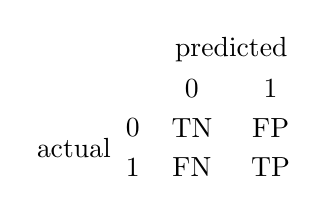
\begin{tikzpicture}
	\node at (1,3) {predicted};
	\node at (0.5,2.5) {$0$};
	\node at (1.5,2.5) {$1$};
	\node at (0.5,2) {TN};
	\node at (1.5,2) {FP};
	\node at (0.5,1.5) {FN};
	\node at (1.5,1.5) {TP};
	\node at (-0.25,2) {$0$};
	\node at (-0.25,1.5) {$1$};
	\node at (-1,1.75) {actual};
\end{tikzpicture}

\caption{confusion matrix}
\end{figure}

\begin{figure}[H]
\centering	
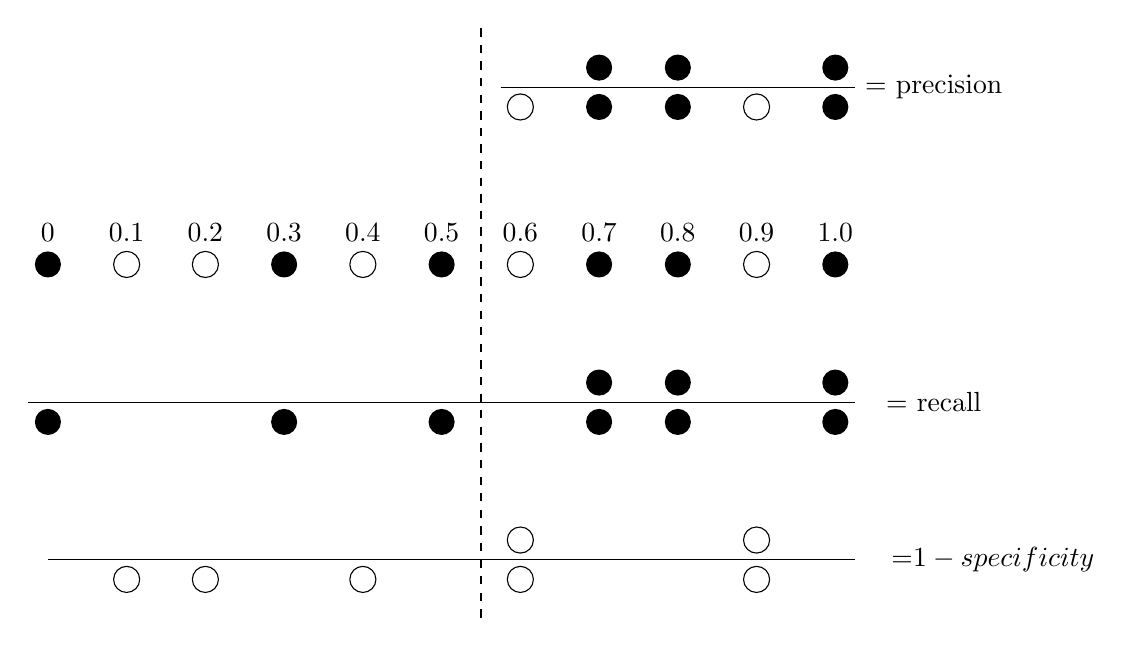
\begin{tikzpicture}
	\node [circle,fill] (s) [label=$0$] at (0,0) {};
	\node [circle,draw] (s) [label=$0.1$] at (1,0) {};
	\node [circle,draw] (s) [label=$0.2$] at (2,0) {};
	\node [circle,fill] (s) [label=$0.3$] at (3,0) {};
	\node [circle,draw] (s) [label=$0.4$] at (4,0) {};
	\node [circle,fill] (s) [label=$0.5$] at (5,0) {};
	\node [circle,draw] (s) [label=$0.6$] at (6,0) {};
	\node [circle,fill] (s) [label=$0.7$] at (7,0) {};
	\node [circle,fill] (s) [label=$0.8$] at (8,0) {};
	\node [circle,draw] (s) [label=$0.9$] at (9,0) {};
	\node [circle,fill] (s) [label=$1.0$] at (10,0) {};
	
	% draw the threshold
	\draw [dashed] (5.5,3) -- (5.5,-4.5);
	
	% draw precision
	\node [circle,draw] (s) at (6,2) {};
	\node [circle,fill] (s) at (7,2) {};
	\node [circle,fill] (s) at (8,2) {};
	\node [circle,draw] (s) at (9,2) {};
	\node [circle,fill] (s) at (10,2) {};
	
	\draw (5.75,2.25) -- (10.25,2.25);

	\node [circle,fill] (s) at (7,2.5) {};
	\node [circle,fill] (s) at (8,2.5) {};
	\node [circle,fill] (s) at (10,2.5) {};
	
	\node at (11.25,2.25) {= precision};
	
	% draw recall
	\node [circle,fill] (s) at (0,-2) {};
	\node [circle,fill] (s) at (3,-2) {};
	\node [circle,fill] (s) at (5,-2) {};
	\node [circle,fill] (s) at (7,-2) {};
	\node [circle,fill] (s) at (8,-2) {};
	\node [circle,fill] (s) at (10,-2) {};
	
	\draw (-0.25,-1.75) -- (10.25,-1.75);
	
	\node [circle,fill] (s) at (7,-1.5) {};
	\node [circle,fill] (s) at (8,-1.5) {};
	\node [circle,fill] (s) at (10,-1.5) {};
	
	\node at (11.25,-1.75) {= recall};
	
	% ROC
	
	\node [circle,draw] (s) at (1,-4) {};
	\node [circle,draw] (s) at (2,-4) {};
	\node [circle,draw] (s) at (4,-4) {};
	\node [circle,draw] (s) at (6,-4) {};
	\node [circle,draw] (s) at (9,-4) {};
	
	\draw (0,-3.75) -- (10.25,-3.75);
	
	\node [circle,draw] (s) at (6,-3.5) {};
	\node [circle,draw] (s) at (9,-3.5) {};
	
	\node at (12,-3.75) {=$1 - \text{specificity}$};
\end{tikzpicture}
\caption{PR and ROC curve}
\end{figure}

\begin{equation}
    \begin{aligned}
	\text{precision} &= \frac{TP}{TP + FP} \\
	\text{recall} &= \frac{TP}{TP + FN} \\
	\text{false positive rate} &= \frac{FP}{FP + TN} \\
    F_1 &= \frac{2}{\displaystyle \frac{1}{\text{precision}} + \frac{1}{\text{recall}}}
    \end{aligned}    
\end{equation}




\cindex{confusion matrix} (\cindex{PR curve}) is a plot between \cindex{precision} and \cindex{recall} (precision is the $y$ axis). There is a trade-off between precision and recall. Given a fixed model and prediction, when the threshold increases, the precision might increase (it could decrease) and the recall will always decrease. Sometimes you may care more about precision, such as classifying safe video for kids. Sometimes you care more about recall, such as the surveillance image classification. For two models, select the one that could embed the other PR curve.




\cindex{receiver operating characteristic} (ROC) is a plot between \cindex{recall} and $1 - \text{specificity}$ (recall is the $y$ axis). The \cindex{area under the curve} (\cindex{AUC}) measures how good a model is. A random classifier will have $\text{AUC} = 0.5$. Compared with ROC curve, PR curve is preferred when:
\begin{enumerate}
	\item positive rate is rare.
	\item care more about false positive than false negative.
\end{enumerate}
















